\section{ECS Literature Review}
\label{chap:1}

Historically, the ECS design pattern was introduced in 1998 with the game titled "Thief: The Dark Project".\cite{RomeoPHD} And the 
motivation behind designing their ECS is that OOP techniques were plaguing the games industry at the time with massive class 
hiearchies, deep inheritance paths, and introduced highly specialized code to projects\cite{Haerkoenen2019}. 
The ECS pattern argues from the position that it can solve all these problems by limiting the hierachy to contain only three layers. It exists as an architectural pattern that follows Data-Oriented-Design (DOD) principles.\cite{RomeoPHD} To this day, the ECS pattern maintains its importance in simulations. In 2015, Apple introduced an implementation of ECS into their GameplayKit API framework. \cite{AppleECS}

Literature on the ECS pattern is limited and hard to find. Although, as mentioned in the abstract there are many articles, conferences, and well-documented libraries from respected individuals in the games industry. GECS is inspired by the articles written by Sander Mertens, the creator of the very popular FLECS framework and can be found in \cite{SanderMertensECS}. 

\subsection{Entity Component System Foundations}
These are the foundational definitions used in this paper. All are based from the FAQ provided by \cite{SanderMertensFAQ} and \cite{RomeoPHD} research.

\subsubsection{Entity}
    An entity is a unique identifier used to represent a "object" in a simulation. This unique identifier is used in some manner by the ECS to collect a set of components. Some ECS's try to make the identifier intelligent to optimize component selection bits in the identifier to store more location information. This will be discussed in the existing ECS implementions.

\subsubsection{Component}
    Generally speaking, a component is data. It can be defined as a struct, tuple, or class. For this thesis, a component is defined as a segment of either complete or incomplete data. This will be discussed in part \ref{chap:3}.

\subsubsection{System}
    A system is a function defined by the ECS user that intends to execute operations over a set of entities. It 
    contains two parts: the query and execution phase. A system queries for a collection and then executes a function 
    that modifies, creates, or destroys the objects of that selection.

\subsubsection{Tick}
    A tick is defined to be a serialization point during runtime in which all systems have been processed and the ECS is
    ready to process them all again. This is the serialization point used in the model.

\subsection{Motivation \& The Weaknessess Of Object Oriented Programming}

% TODO: Sources
It has been exhaustively shown that Object-Oriented Programming increases the difficulty of achieving desired simulation goals and that there are plenty attractive alternatives. The two main weaknesses that an ECS intends to solve is: poor cache utilization and poor parallelization.\cite{RomeoPHD}

Large projects deep into using OOP principles learn how hard it is to keep cached what you need and keep junk out. OOP principles can make pointer abuse very easy and cause the cache to overwrite potentially useful data in the near future. ECS solves this by introducing components. Since components are detached from their entity, we as engine designers can put these components wherever we please. It's not an uncommon practice to see component data be stored in long homogenous vectors. Suppose you have to do a heavy operation across the set of entities that all contain component $Q$. An ECS in this situation will be extremely cache friendly, due to $Q$ being next to components that all contain the same component type.

In OOP, parallelism can be painful due to synchronization errors over memory that was not engineered to effectively be
parallelized. Because ECS follows principles from Data-Oriented Design, an ECS can generally produce code that is more
parallelizable by default\cite{RomeoPHD}. The concept of storing components as homogeneous vectors not only helps with caching but because all data pertaining to a component is already homogeneous -- it's easy to process in parallel or in groups. \cite{Wiebusch2012}\cite{SanderMertensECS}

\subsection{Example Entity-Component System Model}
\label{sec:ecs_naive}
The following section discusses a naive implementation to give some understanding as to how to organize data together. This
naive implementation is not thread safe and is presented as C code.

\subsubsection{Structuring Data}

Below is the members of a hypothetical naive ECS implementation. This implementaion style uses the same style that GECS
uses, called Dense ECS \cite{EnTT_SparseSets}.

\begin{figure}[H]
\begin{lstlisting}[
    language=Java,
    numbers=none
]
struct system {
    void (*run_sys)(ecs *e); /* Fun : user defined sys function */
    map_t components;        /* Map : component -> *Vec : component */
};
struct entity_record {
    map_t component_table;   /* Map : component id -> index */
};
struct ecs {
    int64_t id_gen;          /* Int : generates unique entity ids */
    map_t component_table;   /* Map : component id -> Vec: component */
    map_t entity_table;      /* Map : entity id -> entity_record */
    vec_t systems;           /* Vec : system */
};
\end{lstlisting}
    \caption{Example ECS Members}
    \label{code:naive_ecs_data}
\end{figure}

ECS architecture are built upon two core data structures: vectors and maps. As seen above, it has all the parts an ECS requires to function. When initializaing, \texttt{id\_gen} is set to 0 and increments for each new entity created. The component table maps a given component ID to a vector of that type of component. This vector can then be returned immediately by the ECS to allow for a user to process all entity components of a specific kind with a linear operation and a huge win in cache locality.  

Already, there are many opportunities to parallelize.

\subsubsection{Accessing Single Entities}
In order to create a new entity the following steps are taken to manipulate the data within the structs:

\begin{enumerate}
    \item Load x \(\leftarrow\) \texttt{struct ecs}
    \item Increment \texttt{x.id\_gen}
    \item Return \texttt{x.id\_gen}
\end{enumerate}

In order to perform add, create, modify, or delete operations off of a specific entities component data the \texttt{entity\_record} must be loaded from the \texttt{entity\_table}.

\begin{enumerate}
    \item Load \texttt{x} \(\leftarrow\) \texttt{struct ecs}
    \item Load \texttt{r} \(\leftarrow\) \texttt{x.entt\_table}
    \item Load \texttt{c} \(\leftarrow\) \texttt{r.component\_table}
    \item Perform operation on \texttt{c}
\end{enumerate}

As can be seen in the two algorithms above, a Dense ECS is not for modifying a single entity at a time but many all at once. So, single entity accesses are intentionally slower that component accesses. \cite{EnTT_SparseSets}

\subsubsection{Accessing Components}
A core feature of an ECS implementation is for the ability to query systems based on what components the entities inside the system require. Based on that, each system when registered with the ECS will collect pointers to which component vectors they
are capable of working on. 

When registering a system:
\begin{enumerate}
    \item For each component ID \( \texttt{x} \leftarrow [\ldots] \)
    \item Load ptr \( \texttt{p} \leftarrow \texttt{struct ecs : entity\_table} \) such that \texttt{p} contains the vector for \texttt{x}
    \item Save $(\texttt{x}, \texttt{p}) \rightarrow \texttt{struct system : components}$
\end{enumerate}


When registering a component, notice how there is no component id generator. This implementation offloads the task of id
generation to C having unique types. Using macros, the type name can be sent as a stack allocated string to a function to be digested into a component id. The hashing function used by GECS and this model is djb2 \cite{hashing}, a nice and fast hashing function that has decently low collision probability.

% https://github.com/SanderMertens/ecs-faq
\subsection{Existing ECS And Implementation Styles}
From part \ref{chap:1}, its easy to surmise that the ECS pattern can be implemented in many different ways, giving way to unique performance benefits and tradeoffs per style. This section covers an overview of various implementation styles discovered around ECS architectures.

\subsubsection{Entity ID Styles}
A lot can be done with just reserving a couple bits on IDs generated. The popular ECS framework called FLECS, short for Fast 
Lightweight Entity Component System, proposes to represent all component ID's generated in the same manner entity ID's are generated. Notice how in section \ref{sec:ecs_naive}, the naive ECS contains two different methods of ID generation: hashing component typenames and an ID generator counting up. FLECS splits a \texttt{uint64\_t} into two parts where the lower 32 bits represents the entity and the upper 32 bits are reserved for optimizing internal ECS mechanisms.

\begin{figure}[H]
    \centering
    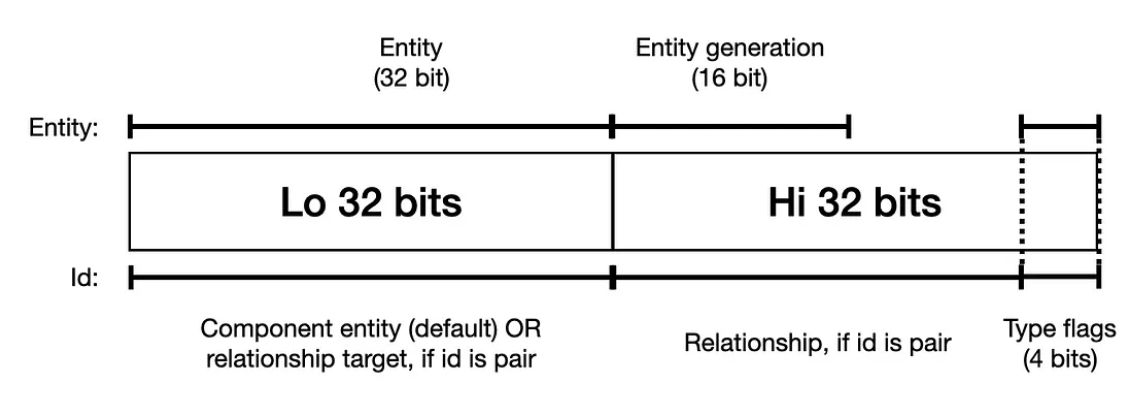
\includegraphics[width=0.5\linewidth]{resources/entity_generation.png}
    \caption{Smart Entity Generation in FLECS}
    \label{fig:entity_generation}
\end{figure}

\textbf{Runtime Tagging:}
A tag in an ECS is a component with no data. Tags are used generally to apply entities to systems without the intent of editing any data based on the tag, but the components adjacent to it. Since components now generate the same way entities
do, entities can now share a direct relationship to a component via runtime tagging as shown in the example below. \cite{RomeoPHD}

\begin{figure}[H]
    \begin{lstlisting}[
        language=Java
    ]
component CloseCircle = world.component();
entity John = world.entity();
entity Mary = world.entity();
entity Brad = world.entity();
CloseCircle.add(John, Mary, Brad);
CloseCircle.each([](entity friend) { /* John, Mary, and Brad */ });
\end{lstlisting}
    \caption{Runtime Tagging Example}
    \label{code:runtime_tagging}
\end{figure}

The code in figure \ref{code:runtime_tagging} on line 5 is when the ID of \texttt{CloseCircle} is modified to contain some direct relationship to the entities $[\texttt{John}, \texttt{Mary}, \texttt{Brad}]$.

\textbf{Reflection:}
The upper 32 bits can be used for reflection. Reflection is the ability to serialize component data out of the ECS. Since entities are also components, its simple to serialize. Serialization can be done by constructing a new component to house components as if it were an entity, similar to the code in Figure \ref{code:runtime_tagging} but if all the entities were components. By doing this, reflection can be achieved with minimal effort. All that is required needed is to iterate over the components reflected as if they were entities.

\textbf{Entity Liveness:}
A core issue with the ECS pattern is that many games will burn through ID's fast. As such, recycling IDs is important part of an ECS implementation. FLECs reserves the first 16 bits of the upper 32 bits of entity identifiers as a generation count. So a counter for the counter of how many times this ID has been recycled. This allows for easy checking if an entity is still alive.  

\textbf{Entity Relationships:}
One of the biggest flaws of ECS architectures is that perfoming direct entity relationship queries is slow and not performant because of how components and entities are organized. By adding relationships to other entities in the ID, query times based become more efficient. For more information on how this is done inside FLECS, which pioneered this techinque, read Sander Merterns article in \cite{SanderMertensEntityIDs}.

\subsubsection{Dense ECS}
\begin{figure}[htbp]
    \centering
    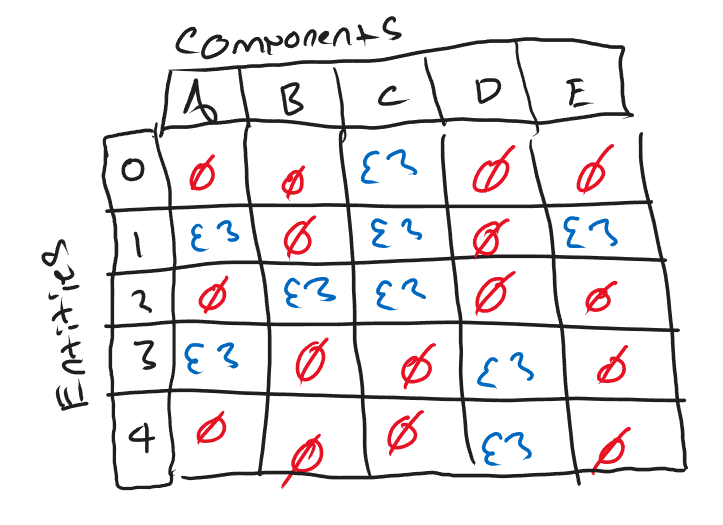
\includegraphics[width=0.5\linewidth]{resources/dense_ecs.png}
    \caption{Dense ECS Architecture Example}
    \label{fig:dense_ecs}
\end{figure}

Dense ECS's, also known as Table based ECS's, store entities inside of large tables. In these tables, components and entities are columns and rows respectively. This gives way to fast component or entity queries, depending on which is is contiguous in memory. Some popular types of this ECS is FLECs or the Unity Game Engine's own ECS, Unity DOTS. \cite{SanderMertensFAQ}

\subsubsection{Sparse ECS}
To understand Sparse ECS architectures, a small introduction into an exotic data structure is necessary. A Sparse Set is a datastructure dedicated to keeping the invariance of the following property:
\begin{equation*}
    \forall v \in \{0,\ldots, n-1\} : \text{D}[S[v]] = v
\end{equation*}
In the property above, $D$ and $S$ represent two vectors. The dense vector and sparse vector respectively. By using these two vectors in unison: lookup, insertion, and deletion time are all $O(1)$ and iteration through the set is $O(n)$. Interestingly enough, this data structure is one that does not require memory to be initialized. \cite{sparse_profit}. The only downside to Sparse Sets is that they must be capable of representing an entire domain since direct index access is used. If, for example $v = 10000$, then there must be at least $10000$ elements in $S$. $D$, the dense vector, will always be the length of the set itself.

The main advantage of sparse ECS implementations is how fast it is to test if an entity contains a component. Because of this, sparse ECS's advantages come in the form of query optimization. In a sparse ECS, a query collects entities by roughly performing an algorithm that queries for all entities that is the union of true values returned from all component sparse sets. Bitset ECS's are known to use similar approaches in their implementations.\cite{EnTT_SparseSets}

There is an alternative use with sparse sets in ECS architectural contexts. Systems could maintain their own sparse sets, which are kept up to date before each tick starts. These sparse sets are used by systems to collect entities related to the system before the system runs itself each tick. An example of an ECS that does this technique is ecst.

Sparse sets also have another use where systems own their own sparse sets and they are kept to date each tick during runtime. These system owned sparse sets are then used to collect entities related to the system. An example of an ECS that does this technique is ecst. \cite{ecst}

Overall, it's important to know that sparse set ECS's are popular in situations where fast add/remove of single component operations are preferred over efficient batch operations. To back this claim, FLECS which is a popular dense ECS published its own benchmarking data against other industry-wide used ECS's. From their data, FLECS has slower add/remove component operations than EnTT, a popular sparse set based ECS.\cite{FLECS_EnTTCompare} Regardless of the advantages and disadvantages of using sparse vs dense ECS's, it can be summed up nicely by the creator of EnTT \cite{EnTT_archetype_and_quote}:

\begin{quote}
    \textbf{It’s a matter of taste}, in fact.
        - Michele Caini
\end{quote}

\subsubsection{Bitset-based}
Another exotic structure used in ECS implementations are bitsets. A bitset is analogous to a hashset. It tracks if certain indices exist are within a set, but the implementations differ vastly however. Bitsets are known for their memory efficiency and are preferred over hashsets if the set is known to store large volumes of objects in the set. \cite{Sutherland2014}

A bitset-based ECS stores components in contiguous arrays where the entity id is used to index. The bitset is used in this application to check if the entity contains that component. There are many different flavours of approaches using this style, such as using a hierarchical bitset structures. \cite{SanderMertensFAQ} EntityX is one of the architectures reviewed that uses bitsets.

\subsubsection{Reactive}
A reactive ECS is more different than the others in this list. A reactive ECS uses signals emitted from mutating entities to keep individual lists of which entities belong to which system. Entitas is an example of this. \cite{SanderMertensECS}

\subsection{Concurrency in ECS Implementations}
The majority of ECS implementations investigated had concurrency support but were severely undocumented. So only two were investigated: FLECS and EnTT.

\subsubsection{FLECS}
The concurrency model of FLECS is simple. The user initially sets the amount of worker threads manually, and entities matched with a system will be divided equally accross threads. Changes to entities are stored in what Sander Mertens calls a "command queue" that are later merged before the end of the tick.\cite{missing_docs} This system is similar to the concurrency model I used for GECS most likely because both GECS and FLECS are Dense ECS's that rely on vectorizing type compositions for concurrency gains.

\subsubsection{EnTT}
The EnTT framework does not do anything special to for concurrent performance gains since their design naturally allows for parallelizable code to be threaded by the user themselves. Michele Caini states in his documentation that "Views, groups, and interators in general aren't thread safe by themselves" but then gives suggestions on how to apply concurrency using their architecture. The author also ends on a note saying that they at least support concurrent entity generation by setting the \texttt{ENTT\_USE\_ATOMIC} flag.\cite{EnTT_multithreading}